\documentclass[conference]{IEEEtran}
\IEEEoverridecommandlockouts
% The preceding line is only needed to identify funding in the first footnote. If that is unneeded, please comment it out.
\usepackage{cite}
\usepackage{amsmath,amssymb,amsfonts}
\usepackage{algorithmic}
\usepackage{textcomp}
\usepackage{xcolor}
\usepackage{flushend}
\usepackage[dvipdfmx]{graphicx}
\ifCLASSOPTIONcompsoc
    \usepackage[caption=false, font=normalsize, labelfont=sf, textfont=sf]{subfig}
\else
\usepackage[caption=false, font=footnotesize]{subfig}
\fi

\def\BibTeX{{\rm B\kern-.05em{\sc i\kern-.025em b}\kern-.08em
    T\kern-.1667em\lower.7ex\hbox{E}\kern-.125emX}}
\begin{document}

\title{Fake News Detection with Generated Comments for News Articles% *\\
% {\footnotesize \textsuperscript{*}Note: Sub-titles are not captured in Xplore and
% should not be used}
% \thanks{Identify applicable funding agency here. If none, delete this.}
}

\author{
    %1st
    \IEEEauthorblockN{Yuta Yanagi}
    \IEEEauthorblockA{\textit{Department of Informatics} \\
        \textit{University of Electro-Communications}\\
        Tokyo, Japan \\
        yanagi.yuta@ohsuga.lab.uec.ac.jp}
    \\
    %4th
    \IEEEauthorblockN{Yasuyuki Tahara}
    \IEEEauthorblockA{\textit{Department of Informatics} \\
        \textit{University of Electro-Communications}\\
        Tokyo, Japan \\
        tahara@uec.ac.jp}
    \and
    %2nd
    \IEEEauthorblockN{Ryohei Orihara}
    \IEEEauthorblockA{\textit{Department of Informatics} \\
        \textit{University of Electro-Communications}\\
        Tokyo, Japan \\
        orihara@acm.org}
    \and
    %3rd
    \IEEEauthorblockN{Yuichi Sei}
    \IEEEauthorblockA{\textit{Department of Informatics} \\
        \textit{University of Electro-Communications}\\
        Tokyo, Japan \\
        seiuny@uec.ac.jp}
    \\
    %5th
    \IEEEauthorblockN{Akihiko Ohsuga}
    \IEEEauthorblockA{\textit{Department of Informatics} \\
        \textit{University of Electro-Communications}\\
        Tokyo, Japan \\
        ohsuga@uec.ac.jp}
}

\maketitle

\begin{abstract}
Recently, fake news is shared via social networks and makes wrong rumors more diffusible.
This problem is serious because the wrong rumor sometimes make social damage by deceived people.
Fact-checking is a solution to measure the credibility of news articles.
However the process usually takes a long time and it is hard to make it before their diffusion.
Automatic detection of fake news is a popular researching topic.
It is confirmed that considering not only articles but also social contexts(i.e. likes, retweets, replies, comments) supports to spot fake news correctly.
However, the social contexts are naturally unavailable when an article comes out, making early fake news detection by means of the social context useless.
We propose a fake news detector with the ability to generate fake social contexts, aiming to detect fake news in the early stage of its diffusion where few social contexts are available.
The fake context generation is based on a fake news generator model. 
This model is trained to generate comments using a dataset which consists of news articles and their social contexts.
In addition, we also trained a classify model.
This used news articles, real-posted comments, and generated comments.
To measure our detector’s effectiveness, we examined the performance of the generated comments for articles with real comments and generated ones by the classifying model.
As a result, we conclude that considering a generated comment help detect more fake news than considering real comments only.
It suggests that our proposed detector will be effective to spot fake news on social networks.
\end{abstract}

\begin{IEEEkeywords}
fake news, disinformation, neural network, natural language processing, deep-learning, microblogs
\end{IEEEkeywords}

\section{Introduction}
In this era, social media is one of the important parts of our lives.
Social media makes it easier to get news and share them with friends online.
However, there is also information with less credibility.
Some of them have misinformation that is made by malicious purposes.
We call them ``fake news''.

\begin{figure}[!t]
    \centering
    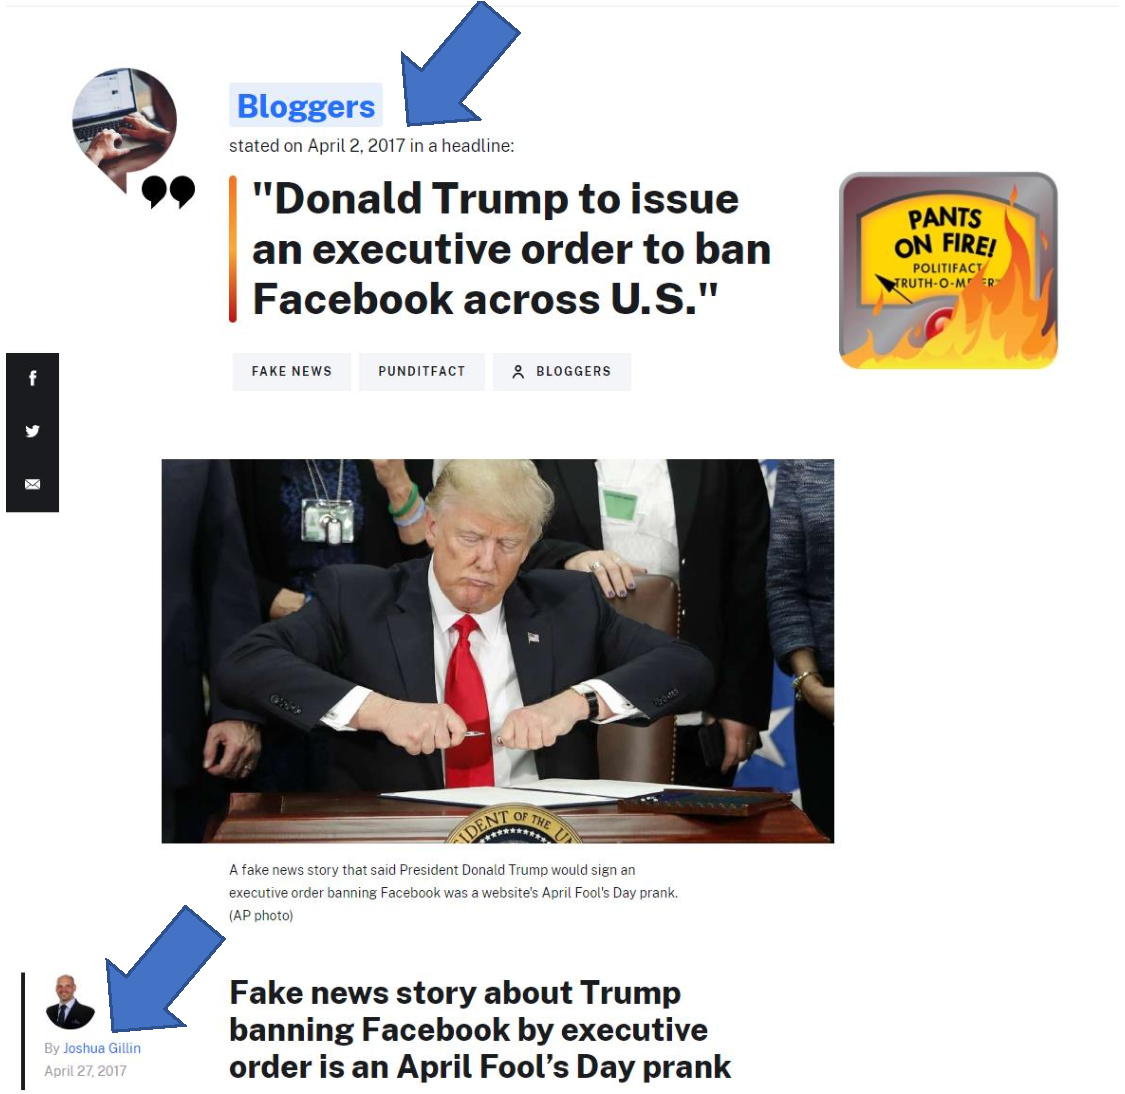
\includegraphics[width=\linewidth]{fact-check.pdf}
    \caption{
        An example of fact-checking. It is confirmed as an April Fool's prank.
        The blue arrows show the posted date of the fake news and the fact-checking result.
        It takes 25 days for the news to be verified as \textit{fake}.
        }
    \label{fig:example}
\end{figure}


Fake news tries to make false rumors diffusible by being shared.
This year, there is so much fake news on COVID-19 and sometimes make wrong rumors in the social networks.
Directer-General of the WHO called this problem ``infodemic'' and he told that fake news is shared faster and more easily than the virus itself\cite{ZAROCOSTAS2020676}. 
Besides, fake news created some not only online, but also offline (real incidents)
e.g. in Washington D.C., fake news on the Pizzagate conspiracy is reported to have motivated the shooting\cite{agencies_2016}.
Nowadays, fact-checking is the most used method to spot fake news.
This is a process of evaluating news by people who have knowledge of news topic.
Fig. \ref{fig:example} is an example of fact-checking\cite{gillin_2017}.
However, this takes so long that it is hard to spot a piece of fake news before it is shared.
Fake news also shakes the premise of democracy due to people cannot get accurate information.
Therefore, researches try to detect fake news through machine learning.

The challenge of this work is there are news articles which try to deceive readers on purpose
and this makes it harder to classify them by a simple rule-based method.
Trying to supplement information for detection,
there are some works which aggregate social context(i.e. retweet, like, and comments)
report better results than considering news text only\cite{Guo:2018:RDH:3269206.3271709}.
However, social contexts are unavailable before being shared.
Hence, there is also a work that generates words likely to be appeared in comments from the news by CVAE to detect fake news when they are just posted\cite{ijcai2018-533}.
Although their work tries to generate comments, they have only achieved to produce words that have a high probability of appearing in the comments.

In this work, we will propose a generation model that evaluates news credibility by news text and generated comments.
This model is modified from generating fake news articles\cite{NIPS2019_9106} and this model learns not only news features but also how to generate comments.
In training, this sequence includes real posted comments but the test sequence does not use them.
The skill of generating comments help classification in the test data.

We measure the performance of our proposed method by experiments with a real posted dataset.

\section{Related works}
To detect and classify fake news is not a new topic because it is similar to detecting spam\cite{shen2017discovering}, rumor\cite{7023340}, and false advertisement\cite{Huang:2017:DFO:3041021.3054233}.
Following previous works\cite{Shu:2017:FND:3137597.3137600,Ruchansky:2017:CHD:3132847.3132877,Wang:2018:EEA:3219819.3219903},
we define fake news as news that is intentionally fabricated and can be verified as wrong.

\subsection{Detecting fake news}
There are many works which detect fake news based on the news content only.
In-text features, writing styles\cite{DBLP:journals/corr/PotthastKRBS17} and amount of emotions\cite{DBLP:journals/corr/abs-1903-01728}
were considered as promising features because commonly fake news has unique styles and emotions.
Besides, using deep neural networks achieved better results in classification on previous works\cite{wang-2017-liar,karimi-tang-2019-learning,karimi-etal-2018-multi}.

Many works consider the social context of news content.
The social context features are generated by user-based\cite{Castillo:2011:ICT:1963405.1963500,8397048,DBLP:journals/corr/abs-1904-13355}, 
post-based\cite{Yang2019UnsupervisedFN,Tacchini2017SomeLI,Jin:2016:NVE:3016100.3016318},
 and network-based\cite{Wu:2018:TFF:3159652.3159677,DBLP:journals/corr/abs-1902-06673}.

Considering the social context, the detection must wait for a while from posting of an article because social contexts are made by users who are exposed to the article.
Therefore, the Two-Level Convolutional Neural Network with User Response Generator(TCNN-URG) was proposed\cite{ijcai2018-533}.
This generates comment by hidden variables which are trained by a probability distribution of comments appearance.
Generated comments can give additional information to classify posts and the model is available even if the news is just posted.
However, the TCNN-URG generates only words that have a high probability of appearing in a comment and it generates no grammatical elements.

\subsection{Generating fake news}
\label{subsec:generate}
In generating natural language articles, the Grover model made natural neural fake news articles\cite{NIPS2019_9106}.
This model is trained by a news dataset where news articles are organized in fields such as news domain, author, posted date, title, and article.
The model was evaluated by the performance of the prediction of one of the news elements.
An interesting finding made by them is that human beings are more likely to be fooled by generated articles than by real ones.
We tried to extend this model and generate natural comments.
\section{methodology}
As we saw in \ref{subsec:generate}, the original Grover model was trained by a news dataset which had five parts.
Each part is attached start and end tokens.
After the training, data without the tags are given to evaluate prediction performance.
We replaced the fields other than the article with three comments and tried to predict one of the comments from the other fields.
We modeled the generation model by the joint distribution like the original one:
\begin{equation}
    \label{eq:joint_distri}
    p = (\rm{article}, \rm{comment\_1}, \rm{comment\_2}, \rm{comment\_3})
\end{equation}
This model's diagram is shown in Fig. \ref{fig:method}.
Basically it was constructed by replacing fields in Grover model’s news structure with comments, except for article.
The purpose of our model was to generate not articles but comments likely to be written by humans.

\begin{figure*}[!t]
    \centering
    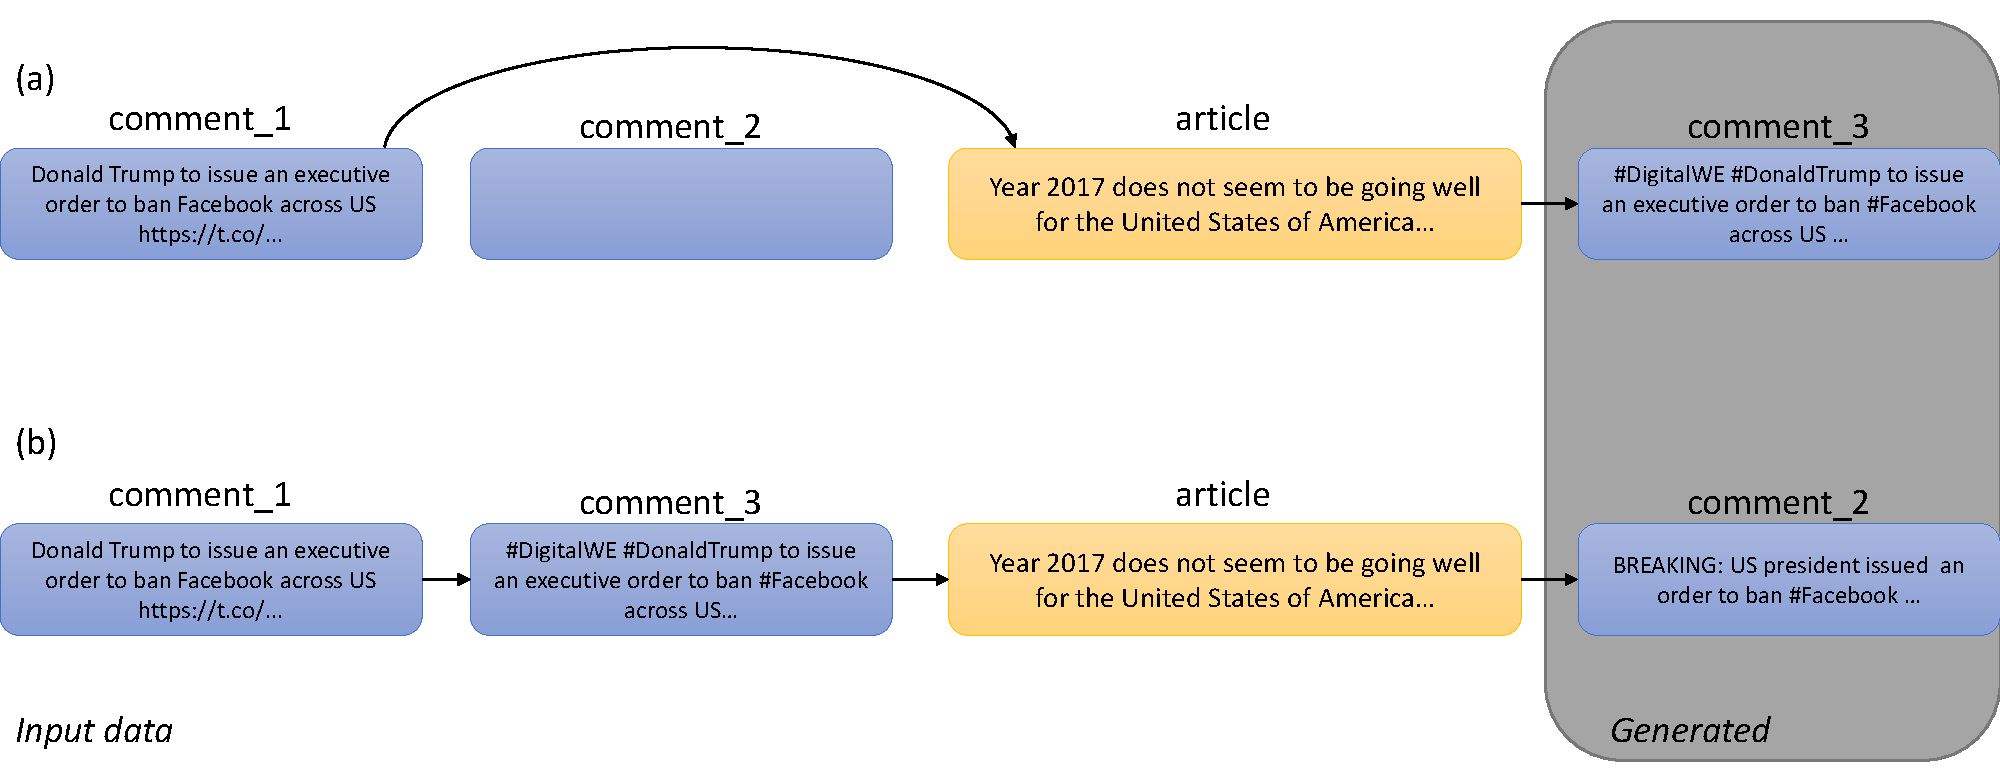
\includegraphics[width=\linewidth,pagebox=cropbox,clip]{fig_method.pdf}
    \caption{
        Two cases of comment generation with our proposed model. 
        (a) shows a case where a comment was generated from an article and a real-posted comment. 
        (b) shows another case where a comment was generated from data that includes the generated comment in (a).    }
    \label{fig:method}
\end{figure*}

The last token of integrated news fields was \texttt{[CLS]} and this was used for classification into real/fake.
This is a same method as for GPT-2\cite{Radford_GPT2}.
The original one was made for the generation of fake news but our proposed model was arranged to generate comments.
Fig.\ref{fig:process} shows our process of experiment.

\begin{figure*}[!t]
    \centering
    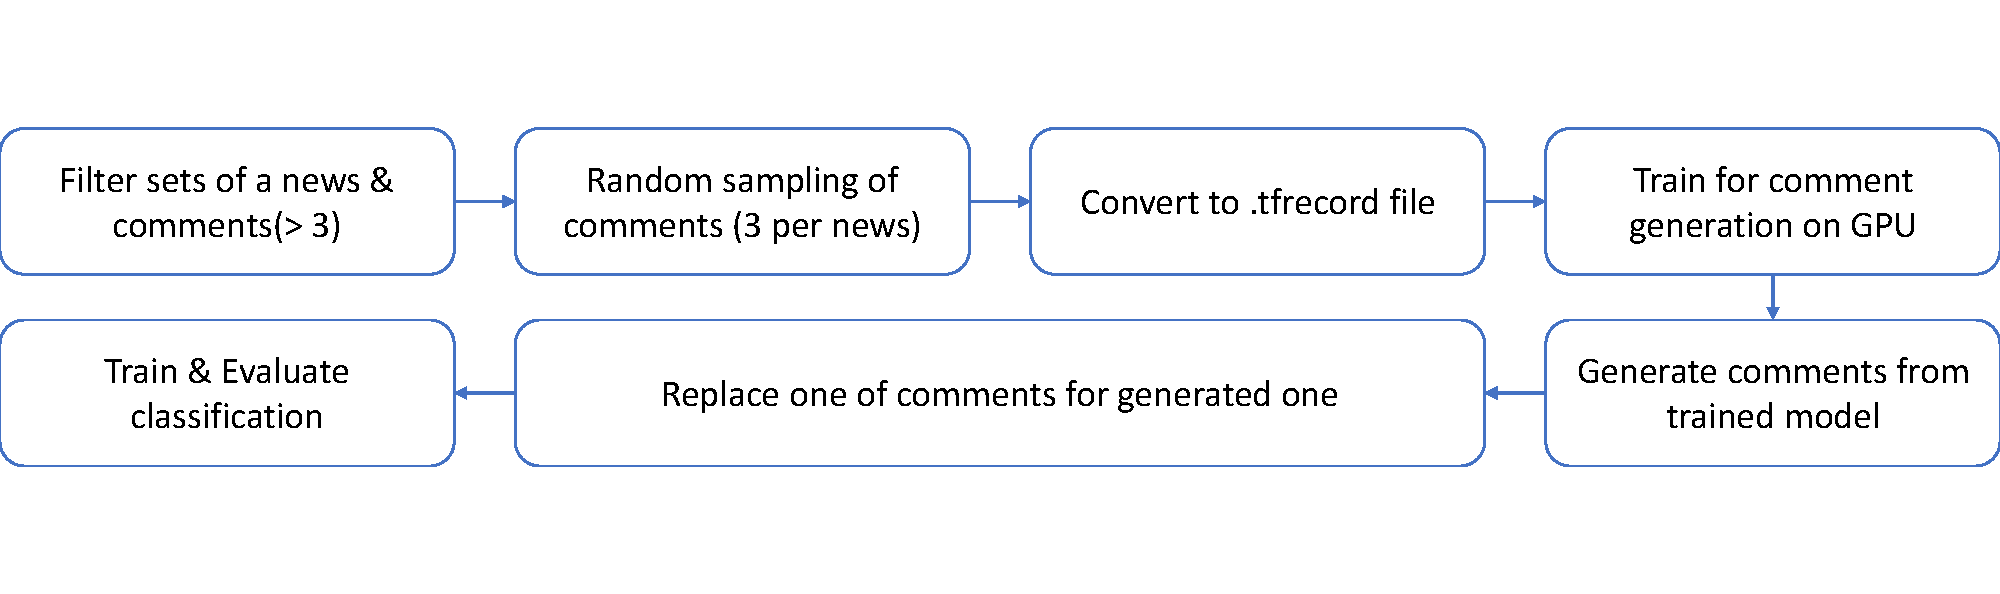
\includegraphics[width=0.8\linewidth,pagebox=cropbox,clip]{fig_process.pdf}
    \caption{The process of our experiment.}
    \label{fig:process}
\end{figure*}

\section{results}
\subsection{Word generation tendency}
\label{subsec:trend}
First of all, we investigated the difference between generated comments from real and fake news.
We generated comments which refer to news articles that are fact-checked by PolitiFact from the FakeNewsNet dataset\cite{Shu2018FakeNewsNetAD}.
This dataset contains sets of a news article and tweets(comments) which refer to it.
We chose news articles which have at least three tweets and sampled three tweets for comment generation.
We prepared 200 sets of news articles and comments for each of the real and fake classes and trained the model to generate comments.
We used the following indexes to evaluate words appeared in the generated comments:
the number of the occurrence of the words(shown in percentage),
ratio of the word's occurrence among the total number of words,
and the difference between the percentages for real and fake classes.
We converted all alphabets to the lowercase letter.
We removed the following elements: stop words provided by NLTK\cite{bird-loper-2004-nltk}, 
url(starts with \textit{http}),
 and symbols such as quotation, period, comma, and so on in order to investigate the frequency of not symbols but words accurately.
On the other hand, we spared mentions, colons, and hashtags(i.e. @anyone, analyze:, \#anything)
 because the addition of these symbols serves different purposes in the social networks.
We found the following by the analysis of the generated comments:
\begin{itemize}[\IEEEsetlabelwidth{3}]
    \item The most frequent word was ``via''(approx. 1.5\%) in the aggregated frequency in real and fake.  
    \item The second and third were ``trump'' and ``obama'' however both of their percentages were under 1\%.
\end{itemize}
We also found the following from the difference between generated comments from real and fake news.
\begin{itemize}[\IEEEsetlabelwidth{3}]
    \item The word ``via'' was also the top frequency of generated word from both real and fake. 
    \item The percent of the frequency of ``via'' in generated comments from fake news article was twice as much as ones from real news.
    \item The word ``via'' was also the word with the largest margin of the percentages between real and fake classes. 
    The margin was approx. 0.9 point.
    \item The word ``breaking:'' was the word with the second-largest margin of the percentages between real and fake classes, 
    where one for the fake was more than the real. 
    The margin was approx. 0.7 point.
\end{itemize}
\subsection{Quality of classification}
We measured the effect of generated comments for classification by comparing classification results with and without the generated comments.
We prepared baselines: classification with the news article only, and with the article and two real-posted comments.
In this experiment, we used pairs of an article of
GossipCop, another data available in the FakeNewsNet dataset, and tweets referring it instead of PolitiFact because the latter has too few data to make the experiment meaningful.
We sampled the same rule as \ref{subsec:trend} although we collect 2000 sets each for the real and fake classes.
The result of classification is Table \ref{tbl:classify_results}.
Our proposed method achieved the best recall score however in precision it was outperformed by models that disregard the generated comments.
On the whole, the generated comments seemed to be not accurate in grammar.

\begin{table}[!t]
    \renewcommand{\arraystretch}{1.3}
    \caption{Results of classification}
    \label{tbl:classify_results}
    \centering
    \begin{tabular}{lccc}
    \hline
    Model name           & Precision & Recall & F1 score \\ \hline
    Article only         & 0.647     & 0.615  & 0.631    \\
     + Real comment * 2  & \textbf{0.682}     & 0.750  & \textbf{0.714}    \\
     + Generated comment & 0.590     & \textbf{0.790}  & 0.675    \\ \hline
    \end{tabular}
    \end{table}
\section{discussion}
\subsection{Generating comments}
According to trends of words in generated comments,
our proposed method seemed to be trained by the topics of news articles.
Most of the generated comments referred to topics of politics and this may be caused by the character of the dataset.

An interesting word in the generated comments is ``breaking:''.
Our experimental results showed that the word was generated more by fake news than real news.
The phenomenon was not reported in the research of TCNN-URG\cite{ijcai2018-533}.
Their research claimed that ``!'', ``?'', ``false'', and so on were important signals of fake news.
"Breaking:" maybe also signal of fake news.

The grammatical quality of the generated comments was clearly poor.
This is caused by a lack of dataset scale. 
Grover model was built using 120 gigabytes of dataset\cite{NIPS2019_9106}.
We need to search or get a larger dataset of articles and tweets.

\subsection{classification}
According to TABLE \ref{tbl:classify_results}, our proposed model achieved the best recall score however in precision its performance was worst.
This means the proposed model can detect more fake news than another model which disregards generated comments even if available social contexts are limited. 

The trend suggests that this model helps people who search for news which require fact-checking. 
However, the model also detected more false fake news than another one therefore we need to make an improvement.
We will check if the trend is changed by using a larger dataset.

\appendix[Settings of experiments]
\label{app:settings}
\begin{itemize}[\IEEEsetlabelwidth{3}]
    \item Trained on Ubuntu 16.04 on Docker in Linux server with TITAN X (Pascal).
    \item Our proposed model was extended from Grover repository by forking on GitHub.
    \item Model size was Grover-Base but we reduced vocabulary a little bit in order to fit for the extension.
\end{itemize}

\section*{Acknowledgement}
This work was supported by JSPS KAKENHI Grant Numbers JP17H04705, JP18H03229, JP18H03340, JP18K19835, JP19K12107, JP19H04113.

\bibliographystyle{IEEEtran}
\bibliography{IEEEabrv,myreferences}

\end{document}
